\documentclass[11pt]{article}

\usepackage[margin=1in]{geometry}
\usepackage{amsmath,amssymb}
\usepackage{graphicx}
\usepackage{hyperref}
\usepackage{booktabs}
\usepackage{enumitem}
\usepackage{xcolor}

\hypersetup{
    colorlinks=true,
    linkcolor=blue,
    citecolor=blue,
    urlcolor=blue
}

\title{Balloon and Aerial Platform Options for Detecting\\
Heavy Neutral Lepton Decays via Atmospheric Cherenkov Light}
\author{N.\ Kamp}
\date{\today}

\begin{document}
\maketitle

\begin{abstract}
We assess platform options for a Cherenkov camera that would detect
heavy neutral lepton (HNL) decays in the atmosphere, produced by a muon beam
dump at a neutrino factory.  After surveying free-flying super-pressure
balloons, high-altitude pseudo-satellites, station-keeping balloons,
tethered aerostats, and low Earth orbit (LEO) satellites, we conclude that a
\textbf{tethered aerostat at $\sim$5~km altitude} best satisfies the
near-term requirements of heavy payload capacity, indefinite
station-keeping, and pointing stability.  We also evaluate a
\textbf{LEO satellite constellation} at $\sim$500~km altitude, which
eliminates the neutrino interaction background entirely at the cost of
intermittent coverage and higher expense.  Combined with a
\textbf{horizontal beam dump geometry} that exploits Earth's curvature to
produce a $\sim$250~km decay baseline, these configurations offer
complementary paths to an HNL search instrument.
\end{abstract}

\tableofcontents

%======================================================================
\section{Introduction}
\label{sec:intro}
%======================================================================

A neutrino factory circulates $\sim 10^{22}$ muons over a ten-year
lifetime~\cite{IDS-NF}.  When the muon beam is directed into a target
(beam dump), the deep-inelastic scattering process $\mu + N \to N_4 + X$
can produce heavy neutral leptons (HNLs, denoted $N_4$) with masses up to
tens of GeV.  The HNL production cross section scales as $|U_{\mu4}|^2$,
the muon-flavor mixing parameter squared.

If the HNLs are produced inside the Earth (i.e.\ the beam is directed
upward or horizontally through rock), they travel essentially unimpeded
through rock and emerge into the atmosphere, where they decay:
\begin{equation}
  N_4 \to \mu^- \pi^+,\quad
  N_4 \to \mu^- \mu^+ \nu_\mu,\quad
  N_4 \to \nu_\mu\, e^+ e^-,\quad \ldots
\end{equation}
The charged decay products --- muons, pions, electrons --- traverse
the atmosphere at relativistic speeds and emit Cherenkov radiation at
optical/near-UV wavelengths.  An imaging Cherenkov camera elevated above
the densest layers of the atmosphere can detect this light.

This concept is analogous to the detection strategy pursued for
upward-going cosmic-ray tau neutrinos by POEMMA~\cite{POEMMA}
and EUSO-SPB2~\cite{EUSO-SPB2-mission}, and for cosmic-ray
optical Cherenkov signals by PBR~\cite{PBR-mission}.  The critical
difference is that the HNL signal is \emph{beam-induced}, so the
detector must be stationed at a known position relative to the beam dump
for an extended period.  This imposes stringent requirements on the
aerial platform: heavy payload capacity (the camera is $\sim$350--900~kg),
precise station-keeping, and long flight duration.

The remainder of this note surveys the available platforms
(Sections~\ref{sec:detector}--\ref{sec:platforms}), argues that a tethered
aerostat is the best near-term solution (Section~\ref{sec:tethered}),
introduces a horizontal beam geometry that exploits Earth's curvature
(Section~\ref{sec:geometry}), evaluates LEO satellites as a
background-free alternative (Section~\ref{sec:leo}), and outlines the
remaining trade-off studies (Section~\ref{sec:outlook}).


%======================================================================
\section{Detector Technology}
\label{sec:detector}
%======================================================================

The baseline detector is a POEMMA/PBR-style imaging Cherenkov
telescope~\cite{PBR-camera,PBR-optics,POEMMA}.  Its key parameters are
summarized in Table~\ref{tab:detector}.

\begin{table}[h]
\centering
\begin{tabular}{lc}
\toprule
\textbf{Parameter} & \textbf{Value} \\
\midrule
Optical design        & 1.1~m Schmidt telescope \\
Focal-plane sensor    & SiPM array, 2048 pixels \\
Angular resolution    & $\sim 0.2^\circ$ per pixel \\
Wavelength range      & 300--900~nm \\
Field of view         & $\sim 12.8^\circ$ \\
Total mass            & 350--900~kg \\
\bottomrule
\end{tabular}
\caption{Baseline detector parameters, following the PBR Cherenkov camera
design~\cite{PBR-camera,PBR-optics}.}
\label{tab:detector}
\end{table}

The camera is a $\sim$1~m-class Schmidt telescope that images
Cherenkov light onto a focal-plane array of silicon photomultipliers
(SiPMs).  Each pixel subtends $\sim 0.2^\circ$, and the 2048-pixel
focal plane covers a $\sim 12.8^\circ$ field of view.  The SiPMs
are sensitive from the near-UV ($\sim$300~nm) through the near-IR
($\sim$900~nm), matching the spectrum of atmospheric Cherenkov light.
This design has been validated in sub-orbital flight by the
EUSO-SPB2 Cherenkov telescope~\cite{EUSO-SPB2-CT}, and is being
developed for a longer-duration mission by PBR~\cite{PBR-camera,PBR-mission}.

The total instrument mass---including optics, focal plane, structure,
power, and electronics---is estimated at 350--900~kg depending on the
level of engineering optimization.  This mass range is the primary driver
for platform selection.


%======================================================================
\section{Platform Options}
\label{sec:platforms}
%======================================================================

We consider five classes of platforms.  Their key characteristics
are compared in Table~\ref{tab:platforms}.

\begin{table}[h]
\centering
\small
\begin{tabular}{lcccc}
\toprule
\textbf{Platform} & \textbf{Altitude} & \textbf{Payload} &
\textbf{Station-keeping} & \textbf{Duration} \\
\midrule
Super-pressure balloon   & 33~km   & $\lesssim$2500~kg & None (drifts) & Weeks--months \\
HAPS drone               & 20--23~km & 5--25~kg & GPS-guided & Months \\
Station-keeping balloon  & 15--28~km & 25--50~kg & $\sim$50~km drift & Weeks--months \\
Tethered aerostat        & $\leq$5~km & $\leq$1500~kg & Perfect (tethered) & Indefinite \\
LEO satellite (single)   & 500~km  & 500--1500~kg & Orbital (passes only) & 3--5~yr \\
LEO constellation ($\times 10$) & 500~km & 500--1500~kg & Orbital ($\sim$25\% duty) & 3--5~yr \\
\bottomrule
\end{tabular}
\caption{Comparison of platform options.}
\label{tab:platforms}
\end{table}


%----------------------------------------------------------------------
\subsection{Free-Flying Super-Pressure Balloons}
\label{sec:spb}
%----------------------------------------------------------------------

NASA's super-pressure balloon (SPB) program launches zero-pressure and
super-pressure balloons to altitudes of 33--40~km, with payloads up
to $\sim$2500~kg.  These balloons have carried scientific payloads
including the EUSO-SPB2 Cherenkov telescope~\cite{EUSO-SPB2-CT,EUSO-SPB2-mission}
and are the baseline platform for PBR~\cite{PBR-mission}.

\paragraph{Advantages.}
\begin{itemize}[nosep]
  \item Altitude of 33~km places the detector above $>$99\% of the atmosphere,
        minimizing absorption and scattering of Cherenkov light.
  \item Payload capacity ($\leq$2500~kg) is ample for the Cherenkov camera.
  \item Heritage: EUSO-SPB2 and PBR provide direct precedent.
\end{itemize}

\paragraph{Disadvantages.}
\begin{itemize}[nosep]
  \item \textbf{No station-keeping.}  Super-pressure balloons drift with
        stratospheric winds (typically circumpolar trajectories).  The balloon
        cannot be held over a fixed ground position.
  \item Flight duration is limited to weeks or months; the EUSO-SPB2
        flight lasted $\sim$37~hours before an anomaly forced termination.
  \item Launch windows and trajectories are weather-dependent; there is no
        guarantee the balloon will remain within line of sight of the beam dump.
\end{itemize}

For a beam-dump experiment requiring the detector at a known, fixed position,
the lack of station-keeping is a critical shortcoming.


%----------------------------------------------------------------------
\subsection{High-Altitude Pseudo-Satellites (HAPS)}
\label{sec:haps}
%----------------------------------------------------------------------

Solar-powered HAPS drones operate in the lower stratosphere (18--23~km)
and can remain aloft for months.  Two leading examples:

\begin{itemize}[nosep]
  \item \textbf{Airbus Zephyr S/T:} Operates at $\sim$21~km altitude.
        Payload capacity is $\sim$5~kg (Zephyr~S) to $\sim$20~kg
        (Zephyr~T).  Endurance record of 64 days.
  \item \textbf{SoftBank/Aerovironment Sunglider (HAWK30):}
        Operates at $\sim$20~km.  Payload capacity $\sim$10--25~kg.
\end{itemize}

\paragraph{Advantages.}
\begin{itemize}[nosep]
  \item GPS-guided flight allows precise station-keeping over a fixed point.
  \item Long endurance (months).
  \item Stratospheric altitude provides a reasonably clear atmosphere.
\end{itemize}

\paragraph{Disadvantages.}
\begin{itemize}[nosep]
  \item \textbf{Payload capacity is far too low.}  At 5--25~kg, HAPS
        drones cannot carry a 350--900~kg telescope.  This is an
        order-of-magnitude mismatch.
  \item The aircraft structure introduces vibrations that may
        degrade the optical point-spread function.
\end{itemize}

HAPS are ruled out by the payload mass requirement.


%----------------------------------------------------------------------
\subsection{Station-Keeping Balloons}
\label{sec:stationkeeping}
%----------------------------------------------------------------------

A newer class of stratospheric balloons uses altitude control to
exploit wind shear for coarse station-keeping:

\begin{itemize}[nosep]
  \item \textbf{Project Loon / Aalyria (Google):} Super-pressure balloons at
        $\sim$18--25~km that adjusted altitude to ride favorable wind layers.
        Station-keeping accuracy was demonstrated to $\sim$50~km
        radius~\cite{Loon-Nature}.  Payload $\sim$10--15~kg.
        Project Loon was shut down in 2021.
  \item \textbf{Aerostar Thunderhead:} Commercial super-pressure balloons
        operating at 18--28~km altitude.  Payload capacity up to
        $\sim$25--50~kg.  Station-keeping via altitude modulation,
        similar to Loon, with $\sim$50~km accuracy.
\end{itemize}

\paragraph{Advantages.}
\begin{itemize}[nosep]
  \item Provides coarse station-keeping ($\sim$50~km radius) without
        propulsion.
  \item Longer duration than conventional free-flying balloons.
  \item High altitude (18--28~km) reduces atmospheric attenuation.
\end{itemize}

\paragraph{Disadvantages.}
\begin{itemize}[nosep]
  \item \textbf{Payload capacity is too low} (25--50~kg vs.\ the required
        350--900~kg).
  \item Station-keeping accuracy of $\sim$50~km is insufficient for
        precise pointing at a beam-dump target.
  \item Technology is not widely available for custom scientific payloads.
\end{itemize}

Station-keeping balloons are similarly ruled out by the mass constraint.


%----------------------------------------------------------------------
\subsection{Tethered Aerostats}
\label{sec:tethered_option}
%----------------------------------------------------------------------

Tethered aerostats (blimps held aloft by a cable) have been deployed for
military surveillance, telecommunications, and atmospheric research for
decades:

\begin{itemize}[nosep]
  \item \textbf{TCOM 71M / TARS (Tethered Aerostat Radar System):} Deployed
        by the US military along the southern border.  Operates at
        $\sim$4.5~km altitude.  Payload capacity $\sim$1600~kg.
  \item \textbf{Jimu-1 (China):}  Set the record for highest tethered
        aerostat at 9,032~m in 2022, following a 7,003~m flight in 2019.
  \item \textbf{Various military/civilian systems:} Tethered aerostats have
        been used in Iraq and Afghanistan for persistent surveillance,
        carrying radar payloads of 500--1500~kg at 1--5~km
        altitude~\cite{Davidson2012}.
\end{itemize}

\paragraph{Advantages.}
\begin{itemize}[nosep]
  \item \textbf{Perfect station-keeping.}  The tether fixes the aerostat
        at a known position.
  \item \textbf{Heavy payload.}  Systems like TCOM 71M carry $>$1500~kg,
        easily accommodating the Cherenkov camera.
  \item \textbf{Indefinite duration.}  Tethered aerostats operate
        continuously (TARS systems were deployed for years).
  \item \textbf{Power via tether.}  The tether can carry power and data
        lines, eliminating battery/solar constraints.
  \item \textbf{Proven technology} with extensive military heritage.
\end{itemize}

\paragraph{Disadvantages.}
\begin{itemize}[nosep]
  \item \textbf{Low altitude.}  Practical tethered operations are limited
        to $\lesssim$5~km, and most deployments are at 1--5~km.
        The Jimu-1 record of 9~km required extreme engineering.
        The atmosphere below 5~km has significant Rayleigh scattering and
        aerosol extinction.
  \item \textbf{Wind-induced motion.}  The aerostat sways in wind, introducing
        pointing jitter.  For Cherenkov detection (angular resolution
        $\sim 0.2^\circ$), this is manageable with a gimbaled mount,
        but is worse than the pointing stability of a free-flying
        stratospheric balloon above the jet stream.
  \item \textbf{Tether logistics.}  A 5~km tether requires a dedicated
        winch station and has a non-negligible failure probability in
        severe weather.
  \item \textbf{Weather.}  Operations may be interrupted by thunderstorms,
        icing, and high surface winds.  The aerostat must be winched down
        during severe weather.
\end{itemize}


%======================================================================
\section{The Tethered Aerostat Solution}
\label{sec:tethered}
%======================================================================

Despite the altitude limitation, the tethered aerostat is the only
platform that simultaneously satisfies the three core requirements:
\begin{enumerate}[nosep]
  \item \textbf{Payload $\geq$ 350~kg:}  TCOM-class aerostats carry
        $>$1500~kg.
  \item \textbf{Station-keeping:}  The tether provides perfect,
        continuous positioning.
  \item \textbf{Long duration:}  Tethered systems operate for months
        to years.
\end{enumerate}

The low altitude (5~km vs.\ 33~km for an SPB) means the detector sits
within the troposphere, where atmospheric scattering and absorption are
significant.  However, for this experiment the relevant Cherenkov light
is produced by HNL decay products traveling \emph{above} the balloon
(in a downward-looking geometry) or at the same altitude (in a horizontal
geometry).  In either case, the light path through the dense lower
atmosphere can be kept relatively short.

\subsection{Station-Keeping Precision and Wind-Induced Displacement}

While we describe the tethered aerostat as providing ``perfect''
station-keeping, the balloon does not sit motionlessly above the
mooring point.  Wind exerts a horizontal drag force on the envelope,
displacing it downwind --- an effect called \emph{blowby}.  We now
show quantitatively that this displacement has negligible impact on
the physics.

The equilibrium cable angle $\theta$ from vertical satisfies
\begin{equation}
  \tan\theta = \frac{F_{\text{drag}}}{F_{\text{buoy}}}
  = \frac{\tfrac{1}{2}\,\rho_{\text{air}}\,v^2\,C_D\,A}{
          (\rho_{\text{air}} - \rho_{\text{He}})\,V\,g}\,,
  \label{eq:blowby}
\end{equation}
where $v$ is the wind speed, $C_D \approx 0.2$ is the drag coefficient
for a streamlined aerostat, $A$ is the cross-sectional area, $V$ is the
envelope volume, and $g$ is gravitational acceleration.
For a TCOM 71M-class aerostat ($V \approx 18{,}000$~m$^3$,
$A \approx 500$~m$^2$):
\begin{center}
\begin{tabular}{ccc}
\toprule
\textbf{Wind speed} & \textbf{Cable angle $\theta$} &
\textbf{Horizontal displacement at 5~km} \\
\midrule
10~m/s (20~kt)  & $\sim$2$^\circ$  & $\sim$170~m \\
15~m/s (30~kt)  & $\sim$4$^\circ$  & $\sim$390~m \\
20~m/s (40~kt)  & $\sim$8$^\circ$  & $\sim$690~m \\
30~m/s (60~kt)  & $\sim$17$^\circ$ & $\sim$1.5~km \\
\bottomrule
\end{tabular}
\end{center}
Operational protocols require aerostats to be winched down when the
cable angle exceeds $\sim$45$^\circ$, corresponding to sustained
winds above $\sim$60$+$~m/s --- well beyond typical conditions at
inland sites.

\paragraph{Why blowby does not affect the physics.}
Three factors render the $\mathcal{O}(100\text{~m--}1\text{~km})$
displacement negligible:
\begin{enumerate}[nosep]
  \item \textbf{Known position.}  The balloon carries a GPS receiver
        (position accuracy $\sim$1--10~m) and the tether angle is
        continuously monitored.  The instantaneous position is always
        known to $\mathcal{O}(10\text{~m})$, so event reconstruction
        is unaffected.
  \item \textbf{Small compared to the baseline.}  In the horizontal beam
        geometry (Section~\ref{sec:geometry}), the balloon is
        $\sim$250~km from the beam dump.  A 1~km lateral displacement
        is $< 0.5\%$ of the baseline --- negligible for both solid-angle
        coverage and decay-volume calculations.
  \item \textbf{Small compared to the field of view.}  At the
        $\sim$250~km baseline distance, the $12.8^\circ$ camera FOV
        covers $\sim$56~km across.  A 1~km shift in balloon position
        is $\sim$2\% of the FOV width, well within the margin for
        signal acceptance.
\end{enumerate}

In summary, while the tethered aerostat is not rigidly fixed in space,
its position is \emph{known} to meter-level accuracy at all times,
and the wind-induced displacement is negligibly small compared to all
relevant length scales of the experiment.

\subsection{Pointing Stability}

Pointing stability is a separate concern from position.
Wind-induced oscillations of a tethered aerostat at 5~km altitude
have typical amplitudes of $\sim$1--5$^\circ$ on timescales of seconds
to minutes.  Since the Cherenkov camera integrates on nanosecond
timescales (each Cherenkov flash lasts $\sim$10~ns), the relevant
metric is the \emph{instantaneous} pointing, which can be measured
with onboard star trackers or GPS/IMU and corrected in
post-processing.  The $0.2^\circ$/pixel resolution is well matched
to the expected aerostat stability with a passive
gimbal~\cite{Davidson2012,ScrandisDeaconu}.

An interesting precedent is the proposal by Scrandis \& Deaconu to use
a tethered balloon carrying a radio antenna array for cosmic-ray neutrino
detection~\cite{ScrandisDeaconu}.  Their analysis validates the feasibility
of tethered balloon platforms for particle astrophysics at similar altitudes
and payload scales.


%======================================================================
\section{Horizontal Beam Geometry}
\label{sec:geometry}
%======================================================================

A key challenge for HNL detection is maximizing the \emph{decay baseline}:
the distance over which the HNL can decay in the atmosphere (between the
Earth's surface and the detector altitude).  For a vertical beam geometry
--- where the beam is aimed straight up and the detector is directly
overhead --- the baseline is simply the detector altitude $h$.  At
$h = 5$~km, this is quite short, leading to a small decay probability
for long-lived HNLs.

A horizontal beam geometry dramatically extends this baseline by
exploiting the curvature of the Earth.

\subsection{Earth Curvature Geometry}

Consider a beam emerging horizontally from the Earth's surface.
Due to the curvature of the Earth (radius $R_\oplus \approx 6371$~km),
a horizontal line of sight rises above the surface as:
\begin{equation}
  h(d) \approx \frac{d^2}{2 R_\oplus}
  \label{eq:curvature}
\end{equation}
where $d$ is the horizontal distance from the beam exit point and
$h$ is the height above the surface.  Setting $h = 5$~km:
\begin{equation}
  d = \sqrt{2\, R_\oplus\, h}
    = \sqrt{2 \times 6371 \times 5}\;\text{km}
    \approx 252\;\text{km}.
\end{equation}

This means a horizontally aimed beam passes through 5~km of altitude
at a downrange distance of $\sim$250~km.  An HNL traveling along this
beam has $\sim$250~km of flight path through the atmosphere before
reaching the detector altitude --- a factor of $\sim$50 improvement
over the 5~km vertical baseline.

\subsection{Beam Dump Configuration}

In this geometry:
\begin{itemize}[nosep]
  \item The muon beam is aimed approximately horizontally into a
        hillside or underground target.
  \item HNLs produced in the target travel forward along the beam direction.
  \item The HNL trajectory follows a straight line, while the Earth's
        surface curves away beneath it.
  \item After traveling $\sim$250~km, the HNL is at $\sim$5~km altitude
        above the surface.
  \item The tethered aerostat, stationed at 5~km altitude and $\sim$250~km
        downrange, observes the Cherenkov light from HNL decays in the
        surrounding atmosphere.
\end{itemize}

The long baseline means even relatively short-lived HNLs (with decay
lengths of $\mathcal{O}(10\text{--}100)$~km) have significant probability
to decay near the balloon.  Conversely, very long-lived HNLs decay over
the full 250~km path, with decays uniformly distributed along the
trajectory.

Figure~\ref{fig:dump_geometry} shows the available decay region length
as a function of the muon dump length for several dump depths, with
the band in each case spanning balloon heights from 1 to 5~km.
Shallow dumps ($\lesssim$10~m) can access the full $\sim$250~km
baseline even with short muon dump lengths, while deeper dumps
require proportionally longer muon ranges before the beam clears
the surface.

\begin{figure}[ht]
\centering
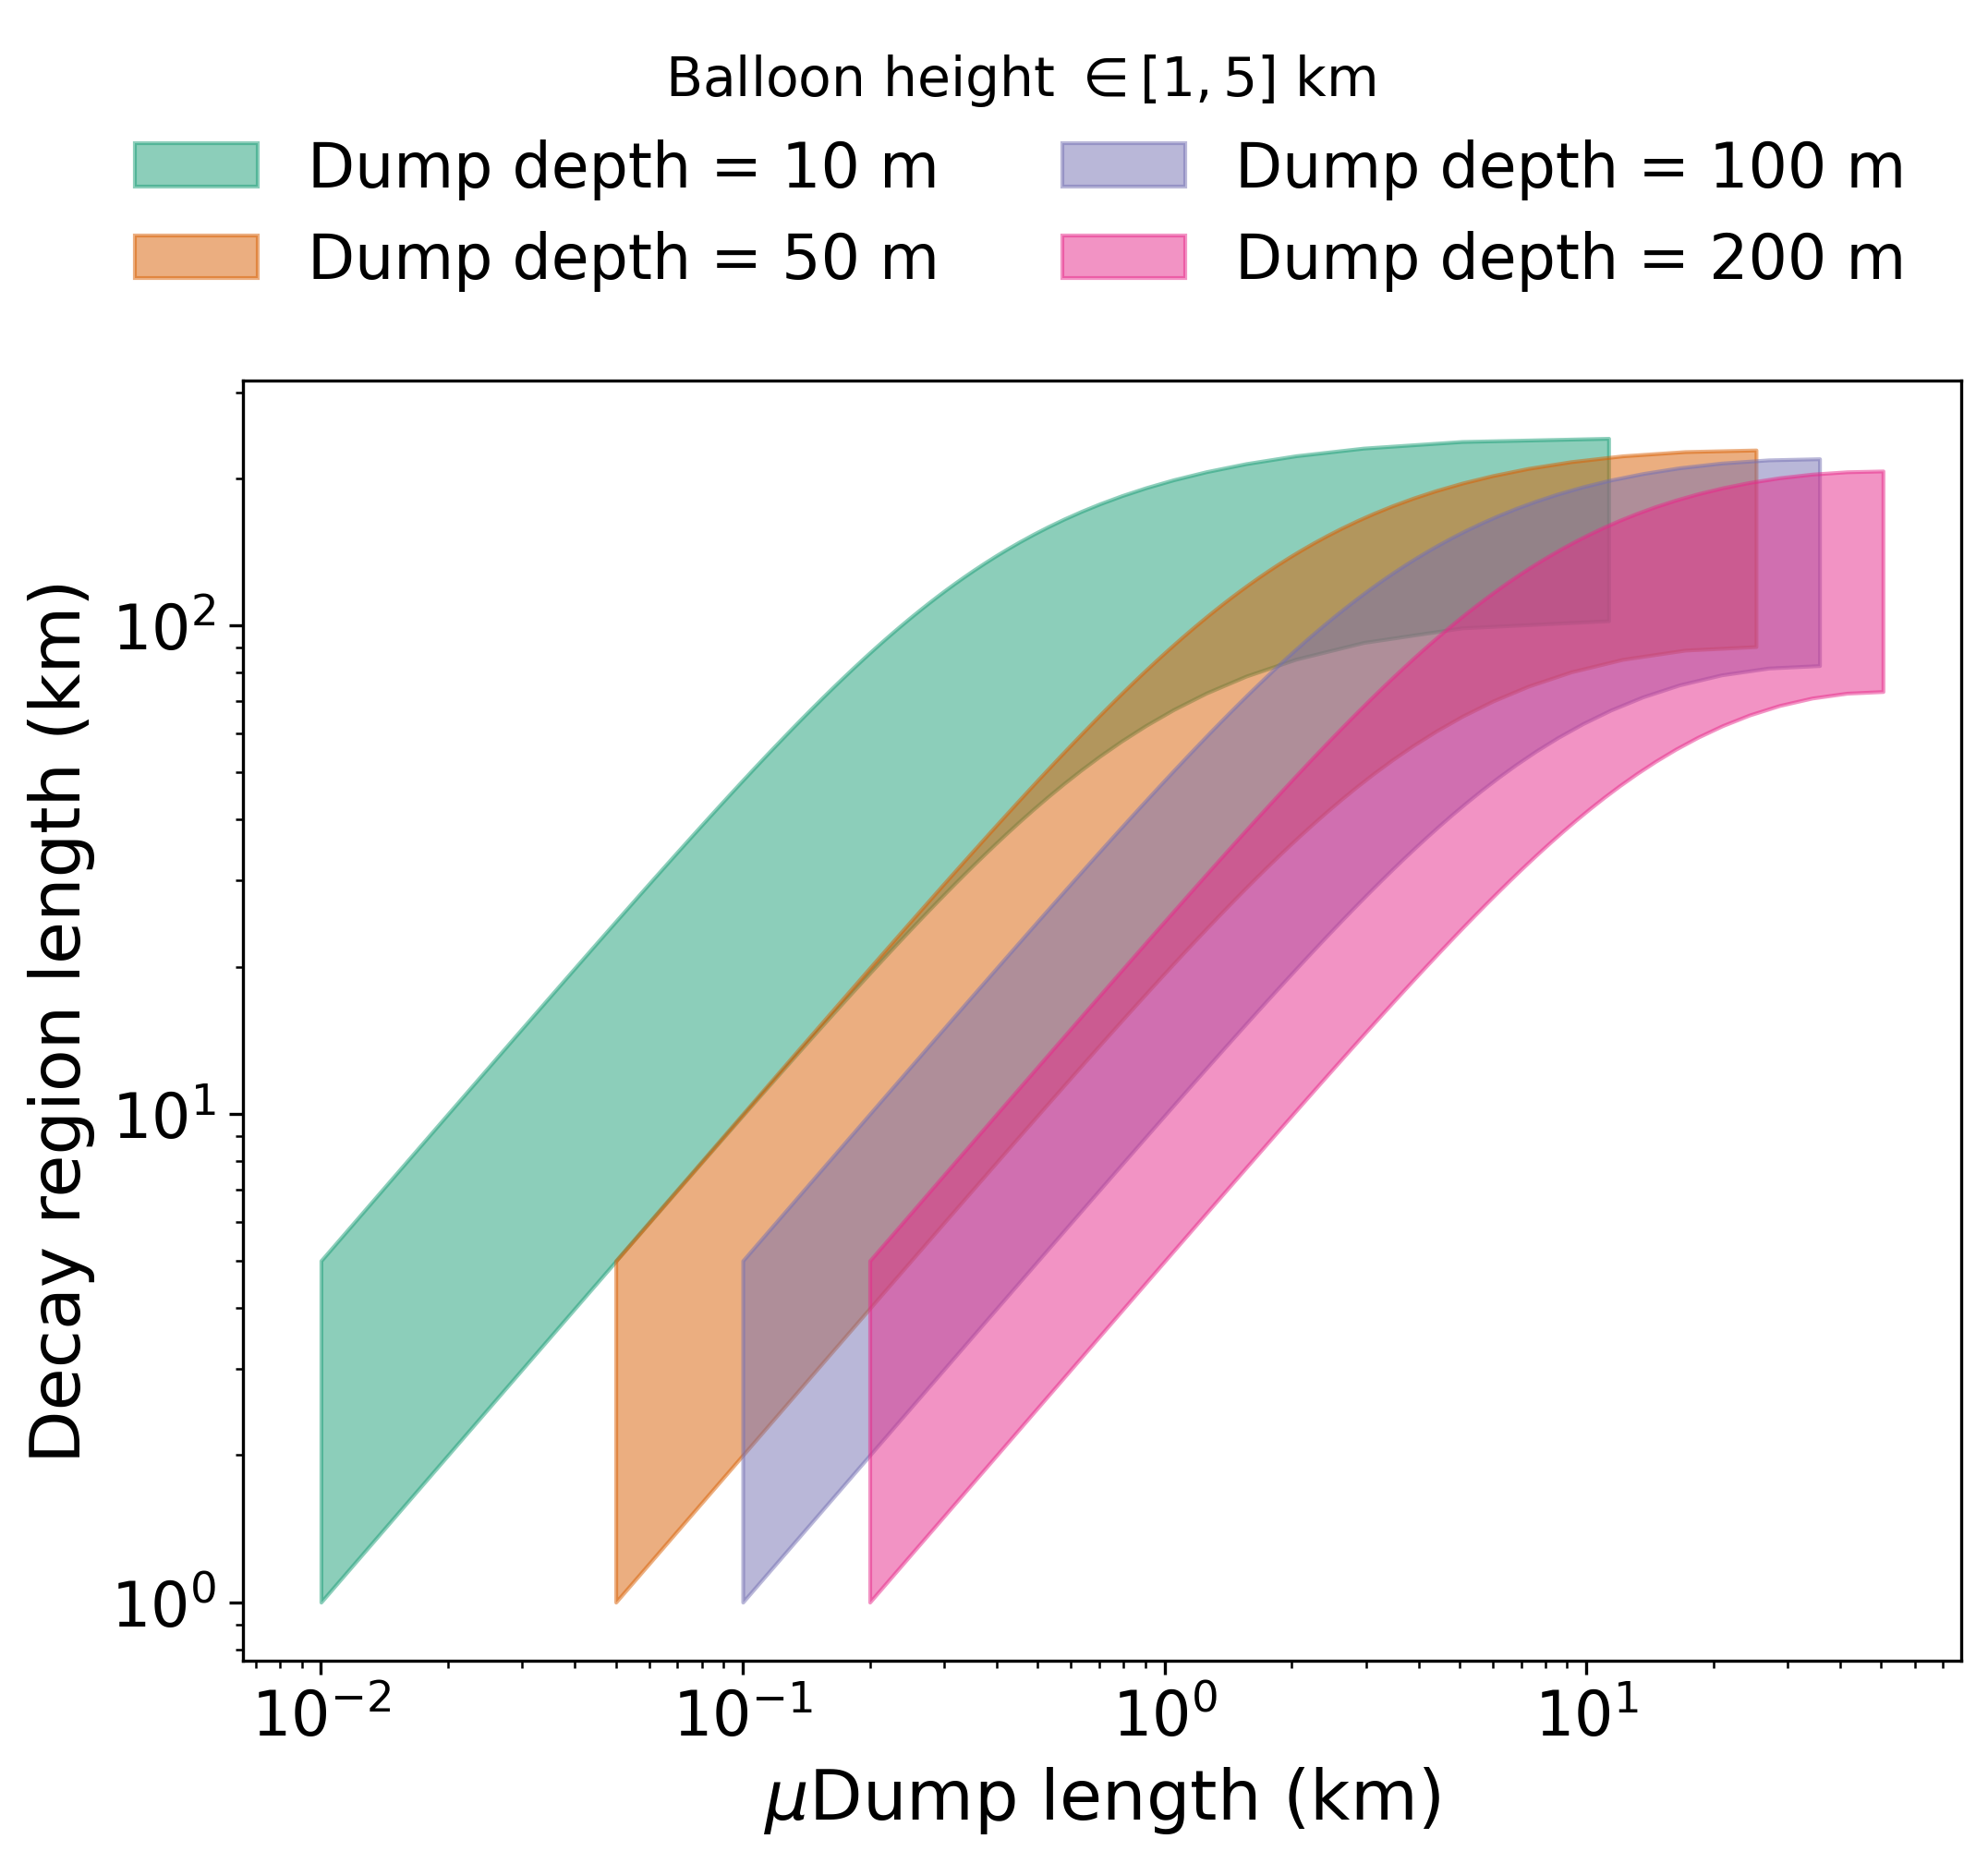
\includegraphics[width=0.75\textwidth]{../Figures/balloon/dump_decay_geometry.png}
\caption{Decay region length vs.\ muon dump length for four dump
depths (10, 50, 100, 200~m).  The shaded bands span balloon
heights from 1 to 5~km.  The upper boundary of each band
($h_{\text{balloon}} = 5$~km) saturates at $\sim$250~km,
set by Earth's curvature via Eq.~\eqref{eq:curvature}.}
\label{fig:dump_geometry}
\end{figure}

\subsection{Atmospheric Considerations}

The horizontal geometry introduces additional atmospheric effects.
Cherenkov light produced at the HNL decay point must traverse the
atmosphere to reach the camera at 5~km altitude.  The Rayleigh
scattering length at sea level is $\sim$15~km at 400~nm, and scales
exponentially with altitude.  For decay altitudes of 3--5~km, the
atmospheric transmission over distances of $\sim$10--50~km is
$\mathcal{O}(10\text{--}50\%)$, depending on wavelength and geometry.
A full treatment requires ray-tracing through the atmosphere,
accounting for the altitude-dependent density profile.


%======================================================================
\section{Low Earth Orbit Satellite Platform}
\label{sec:leo}
%======================================================================

An alternative to balloon-based detection is to place the Cherenkov
camera on a low Earth orbit (LEO) satellite at $\sim$500~km altitude.
At this height the atmospheric column density is negligible: neutrinos
from the beam dump pass through effectively zero target material above
the satellite, eliminating the charged-current interaction background
entirely.  The trade-off is higher cost and intermittent coverage of
the beam dump region.

\subsection{Motivation: Background-Free Detection}

In the horizontal beam geometry (Section~\ref{sec:geometry}), the
neutrino interaction background scales with the atmospheric column
depth traversed by beam neutrinos between the surface and the detector
altitude.  For a nearly horizontal beam with surface exit angle
$\theta_{\text{exit}}$, the slant column depth is
$X \propto (1/\cos\theta_{\text{exit}}) \int_0^h \rho(z)\,dz$, which
remains substantial at balloon altitudes of 2--5~km.  At 500~km,
$\rho(z) \approx 0$ and the background vanishes.

This makes LEO particularly attractive if the signal-to-background
ratio at balloon altitude is unfavorable (${S/B \ll 1}$), as even a
modest signal rate in a background-free environment can yield strong
sensitivity.

\subsection{Telescope Size and Satellite Class}

The baseline PBR-style Cherenkov camera
(Section~\ref{sec:detector}) has a $\sim$1~m aperture and a total
instrument mass of 350--900~kg.  Hosting this on a LEO satellite
requires a spacecraft in the \textbf{1,000--2,000~kg class}.
For reference:
\begin{itemize}[nosep]
  \item \textbf{WorldView-3:} 1.1~m aperture, 2,800~kg total mass,
        617~km altitude~\cite{WorldView3}.
  \item \textbf{NUSES/Terzina} (launching 2026): 430~mm
        Schmidt--Cassegrain with a 640-pixel SiPM focal plane at
        535~km --- a direct pathfinder for space-based Cherenkov
        detection with SiPMs~\cite{NUSES-Terzina}.
  \item \textbf{POEMMA} (proposed): two 4~m Schmidt telescopes with
        hybrid MAPMT$+$SiPM focal planes at 525~km, instrument mass
        $\sim$1,550~kg each~\cite{POEMMA}.
\end{itemize}
A smaller 0.5~m telescope on a $\sim$500~kg satellite is a less
expensive alternative with reduced collecting area.  The Schmidt
optical design is more compact than Cassegrain, and SiPM focal planes
are lighter than CCD/CMOS imagers, both of which help reduce the
required satellite mass.

SiPM radiation damage in the LEO environment is manageable for
$\sim$3-year missions through thermal annealing
protocols~\cite{NUSES-Terzina}.

\subsection{Orbital Coverage of the Beam Dump Region}

The HNL decay region extends $\sim$250~km along the beam axis at
0--5~km altitude.  A satellite at 500~km altitude has a large
instantaneous footprint but passes over any given ground region for
only $\sim$5--10~minutes per pass, with 2--4 passes per day (depending
on orbital inclination and the latitude of the beam dump).

Furthermore, Cherenkov detection requires darkness (the optical
Cherenkov flash must be distinguished from daylight backgrounds),
so only nighttime passes are useful --- roughly half of the total.

Table~\ref{tab:leo_coverage} summarizes the duty cycle as a function
of constellation size.

\begin{table}[h]
\centering
\small
\begin{tabular}{lccc}
\toprule
\textbf{Configuration} & \textbf{Satellites} &
\textbf{Duty cycle} & \textbf{Approx.\ cost} \\
\midrule
Single satellite     & 1  & $\sim$1--3\%  & \$60--215M \\
Stereo pair          & 2  & $\sim$1--3\%  & \$120--430M \\
Moderate coverage    & 10 & $\sim$25\%    & \$200M--1B$^*$ \\
Near-continuous      & 30 & $\sim$75\%    & \$500M--2B$^*$ \\
\bottomrule
\multicolumn{4}{l}{\footnotesize $^*$Mass production could reduce
per-unit costs by 3--10$\times$.}
\end{tabular}
\caption{LEO constellation coverage of the beam dump region
and estimated cost.  Duty cycle accounts for the nighttime-only
constraint.}
\label{tab:leo_coverage}
\end{table}

For reference, the Iridium constellation uses 66~satellites at 781~km
for continuous global communications, and Planet Labs operates
$\sim$200 Dove satellites for daily global imaging.

\subsection{Stereo Reconstruction from Orbit}

Two satellites in the same orbital plane, separated along-track by
$\sim$300~km, provide continuous stereo observation during each
pass over the beam dump region.  This is the configuration adopted
by POEMMA (adjustable 25--1000~km separation) and demonstrated by
the DUSAT mission (two 95~kg satellites at 394~km
separation, $\sim$\$32M total~\cite{DUSAT}).

Using the stereo resolution formulae from
Section~\ref{sec:discrimination} with $D \sim 500$~km,
$B \sim 300$~km, and $\delta\theta = 0.2^\circ \approx 3.5$~mrad:
\begin{align}
  \sigma_\perp &= D \cdot \delta\theta
    \approx 1.75~\text{km}, \\
  \sigma_\parallel &= \frac{D^2\,\delta\theta}{B}
    \approx 2.9~\text{km}.
\end{align}
This is coarser than balloon-based stereo (where $D \sim 10$--100~km)
but sufficient to distinguish events at different altitudes along the
beam and to reject backgrounds from cosmic-ray air showers or other
non-beam sources.

\subsection{Cost Estimates}

For a one-off satellite carrying a 1~m Cherenkov telescope
($\sim$1,500~kg total):
\begin{itemize}[nosep]
  \item \textbf{Satellite bus + instrument:} \$50--200M, depending on
        heritage and level of custom engineering.
  \item \textbf{Launch} (SpaceX Rideshare): \$5--15M for a 1,000--1,500~kg
        payload to LEO~\cite{SpaceX-Rideshare}.
  \item \textbf{Total per unit:} $\sim$\$60--215M.
\end{itemize}

A smaller telescope (0.5~m aperture, $\sim$500~kg satellite) would
cost $\sim$\$20--60M per unit, making a 10-satellite constellation
feasible at \$200--600M --- comparable in cost to a single large
ground-based particle physics detector.

At mass-production scale, standardized satellite buses can reduce
per-unit costs dramatically: Starlink~V2~Mini satellites
($\sim$800~kg) are estimated at \$300--500K each, though these carry
far simpler payloads than a Cherenkov telescope.

\subsection{Tethered Aerostat vs.\ LEO: Trade-offs}

Table~\ref{tab:aerostat_vs_leo} compares the two leading platform
options.

\begin{table}[h]
\centering
\small
\begin{tabular}{lcc}
\toprule
& \textbf{Tethered Aerostat} & \textbf{LEO Stereo Pair} \\
\midrule
Altitude           & 5~km          & 500~km \\
Duty cycle         & $\sim$100\%   & $\sim$1--3\% \\
Background         & Significant   & Negligible \\
Cost (3-year)      & \$14--22M     & \$120--430M \\
Stereo baseline    & 15--30~km     & $\sim$300~km \\
Position resolution & 35--175~m    & 1.75~km \\
Heritage           & TARS (decades) & NUSES/Terzina (2026) \\
\bottomrule
\end{tabular}
\caption{Comparison of the tethered aerostat and LEO stereo pair
for HNL detection.}
\label{tab:aerostat_vs_leo}
\end{table}

The key question is whether the background suppression at LEO
altitude compensates for the $\sim$30$\times$ lower duty cycle and
$\sim$10$\times$ higher cost.  If the signal-to-background ratio at
balloon altitude is favorable ($S/B \gtrsim 1$), the tethered aerostat
is clearly preferred: it is cheaper, provides continuous coverage,
and enables finer spatial reconstruction.  If $S/B \ll 1$ at 5~km,
the background-free LEO environment may be essential --- even a
stereo pair with $\sim$3\% duty cycle would accumulate
background-free signal events over a multi-year mission.

A staged approach is natural: begin with a tethered aerostat to
characterize the signal and background rates, then evaluate whether
LEO is warranted based on the measured $S/B$.  The NUSES/Terzina
mission (2026) will provide critical validation of SiPM-based
Cherenkov cameras in the LEO radiation environment.


%======================================================================
\section{Cost Analysis}
\label{sec:cost}
%======================================================================

A practical assessment of the tethered aerostat approach requires
understanding the costs involved and how they compare to alternative
platforms.

\subsection{Tethered Aerostat Costs}

Cost data for tethered aerostats comes primarily from US military
procurement, where the Tethered Aerostat Radar System (TARS) program
provides the most relevant benchmarks~\cite{TARS-wiki}:

\begin{itemize}[nosep]
  \item \textbf{Unit acquisition:} A complete TARS aerostat system
        (envelope, tether, mooring station, winch, and ground support
        equipment) costs approximately \textbf{\$8--10M} per unit.
  \item \textbf{Annual operations \& maintenance:}  O\&M costs per
        TARS site were $\sim$\$6M/year in fiscal year 1992, reduced to
        $\sim$\$3.5M/year by 2007 through operational efficiencies.
        For a scientific deployment with a smaller support crew, costs
        in the range of \textbf{\$2--4M/year} are plausible.
  \item \textbf{Helium:}  A TCOM 71M-class aerostat requires
        $\sim$20{,}000--40{,}000~m$^3$ of helium.  At current prices
        ($\sim$\$5--15/m$^3$), the initial fill costs
        \$100K--600K, with periodic top-ups needed to compensate for
        diffusion losses.
\end{itemize}

Recent large-scale military contracts provide additional context:
TCOM secured a \$217M contract for Saudi Arabia aerostat platforms
(2021) and a \$979M contract for the Persistent Surveillance
Systems---Tethered (PSS-T) program~\cite{TCOM-PSS-T}.  These figures
include extensive engineering support, spares, and multi-year
operations, and are not directly comparable to a single scientific
deployment.

\subsection{Comparison with Alternative Platforms}

Table~\ref{tab:cost} compares the estimated costs for a 3-year
HNL detection campaign across platform options.

\begin{table}[h]
\centering
\small
\begin{tabular}{lccc}
\toprule
\textbf{Platform} & \textbf{Acquisition} & \textbf{Annual O\&M} &
\textbf{3-Year Total} \\
\midrule
Tethered aerostat       & \$8--10M  & \$2--4M  & \$14--22M \\
NASA SPB campaign       & ---       & \$5--15M/flight & \$10--45M$^*$ \\
HAPS drone              & \multicolumn{3}{c}{(insufficient payload capacity)} \\
Station-keeping balloon & \multicolumn{3}{c}{(insufficient payload capacity)} \\
\bottomrule
\multicolumn{4}{l}{\footnotesize $^*$Assumes 1--3 flights;
no station-keeping guarantee; flight duration uncertain.}
\end{tabular}
\caption{Estimated cost comparison for a 3-year HNL detection campaign.
NASA SPB costs are per flight including integration, launch operations,
and recovery.}
\label{tab:cost}
\end{table}

The tethered aerostat is cost-competitive with a multi-flight NASA
balloon campaign, while offering three critical advantages that have
no price equivalent: guaranteed station-keeping, continuous operation
(vs.\ weather-dependent launch windows and uncertain flight duration),
and the ability to iterate on the instrument without recovering it
from a remote landing site.

\subsection{Comparison with HNL Search Experiments}

To place the tethered aerostat cost in the broader context of the HNL
experimental program, Table~\ref{tab:hnl_cost} compares estimated costs
across current and proposed HNL search experiments.

\begin{table}[h]
\centering
\small
\begin{tabular}{lccl}
\toprule
\textbf{Experiment} & \textbf{Est.\ Cost} & \textbf{HNL Mass Range} &
\textbf{Notes} \\
\midrule
FASER (LHC)   & $\sim$\$2M   & 0.1--2~GeV &
  Reuses LHCb/ATLAS spares~\cite{FASER} \\
Tethered aerostat  & \$14--22M & 1--90~GeV &
  3-year campaign (this work) \\
MATHUSLA (HL-LHC)  & $\sim$\$50M  & 0.5--30~GeV &
  200\,m surface detector~\cite{MATHUSLA} \\
SHiP (CERN SPS)    & $\sim$\$140M & 0.5--8~GeV &
  BDF + detector + beamline~\cite{SHiP-ECN3} \\
DUNE (Fermilab)    & $\sim$\$3.2B  & 0.1--0.5~GeV &
  HNL search is secondary~\cite{DUNE} \\
\bottomrule
\end{tabular}
\caption{Approximate cost comparison of experiments with HNL sensitivity.
FASER cost reflects foundation grants only; CERN provides
infrastructure in kind.  DUNE cost is for the full LBNF/DUNE project,
of which HNL searches are a small fraction of the physics program.
SHiP cost includes the ECN3 facility upgrade ($\sim$60~MCHF),
detector materials ($\sim$51~MCHF), and beamline upgrades
($\sim$14~MCHF).  All costs are approximate and in 2024 USD
(1~CHF~$\approx$~\$1.1).}
\label{tab:hnl_cost}
\end{table}

The tethered aerostat approach occupies a unique cost--performance niche:
\begin{itemize}[nosep]
  \item It is an order of magnitude cheaper than SHiP while probing
        \emph{higher} HNL masses (up to $\sim$90~GeV vs.\ SHiP's 8~GeV
        limit), thanks to the high-energy muon beam at a neutrino factory.
  \item It is comparable in cost to MATHUSLA but accesses the
        muon-mixing sector directly, complementing MATHUSLA's sensitivity
        to HNLs produced in $B$ and $D$ meson decays at the LHC.
  \item Unlike FASER or DUNE, which piggy-back on existing accelerator
        infrastructure, the tethered aerostat requires dedicated deployment
        --- but the total cost remains modest by particle physics standards.
\end{itemize}


\subsection{Cost Drivers and Optimization}

Several factors could reduce the cost of a tethered aerostat deployment
for this experiment:

\begin{enumerate}[nosep]
  \item \textbf{Smaller aerostat.}  If the Cherenkov camera can be
        engineered to the lighter end of the 350--900~kg range, a
        smaller (and cheaper) aerostat envelope may suffice.
        Commercial aerostats in the 500~kg payload class are
        available at lower cost than military TARS systems.
  \item \textbf{Site selection.}  Deploying in a region with mild
        surface winds and infrequent severe weather (e.g.\ high desert
        or polar plateau) would reduce weather-related downtime and
        operational costs.
  \item \textbf{Partnership with military or border surveillance
        programs.}  Piggy-backing the Cherenkov camera onto an existing
        TARS or similar deployment could dramatically reduce costs,
        as the aerostat infrastructure would already be in place.
  \item \textbf{Power via tether.}  Eliminating the need for onboard
        batteries or solar panels simplifies the instrument and
        reduces mass, potentially enabling a smaller aerostat.
\end{enumerate}


%======================================================================
\section{Background Discrimination Strategy}
\label{sec:discrimination}
%======================================================================

The dominant background is neutrino-induced: beam neutrinos from the
same DIS process ($\mu + N \to \nu_\mu + X$) interact in the atmosphere
via charged-current scattering ($\nu_\mu + N \to \mu + X$), producing
muons whose Cherenkov light mimics the HNL signal.  Both signal and
background produce forward-going charged particles with hadronic
activity; at the current level of analysis we treat both as single
Cherenkov tracks weighted by detection probability.

The key physical difference is the \emph{altitude distribution}:
\begin{itemize}[nosep]
  \item \textbf{Background}: The neutrino interaction probability is
        $\propto \rho_{\text{air}}(z) \propto e^{-z/H}$ with scale
        height $H \approx 8.5$~km.  Background events are concentrated
        near the surface.
  \item \textbf{Signal}: HNL decays follow
        $\propto e^{-\ell/L_{\text{decay}}}$ along the beam direction.
        For long-lived HNLs ($L_{\text{decay}} \gg H$), the signal
        altitude distribution is much flatter than the background.
\end{itemize}

We consider three complementary discrimination strategies, implemented
in a two-balloon configuration.


\subsection{Rate Ratio (Two Heights)}

The simplest approach: two balloons at different altitudes
(e.g.\ $h_1 = 2$~km and $h_2 = 5$~km), both at the same downrange
position.  Measure the event rate at each balloon and form the ratio
$R = N(h_1) / N(h_2)$.  The background ratio is fixed by the
atmospheric density profile and is independent of the beam parameters.
The signal ratio depends on $L_{\text{decay}}$ and differs from the
background ratio whenever $L_{\text{decay}} \neq H$.


\subsection{Pixel-Level Spatial Distributions}

Each Cherenkov camera has 2048 pixels at $0.2^\circ$/pixel, covering a
$12.8^\circ$ field of view.  Pointed along the beam direction, different
pixels map to different elevation angles and thus different event
altitudes.  Even a \emph{single} camera provides a 2D spatial
distribution of events on the sky.  A template fit to this distribution
--- with signal and background templates predicted by simulation ---
extracts more information than the integrated rate alone.


\subsection{Stereo Reconstruction}

Two cameras separated by a horizontal baseline $B$ observe the same
event at different pixel positions.  The parallax gives the distance to
the event, enabling full 3D reconstruction.  The position resolution
depends on the angular resolution $\delta\theta$ per pixel, the
distance $D$ to the event, and the stereo baseline $B$:
\begin{align}
  \sigma_\perp &= D \cdot \delta\theta
  \label{eq:sigma_perp} \\
  \sigma_\parallel &= \frac{D^2 \cdot \delta\theta}{B}
  \label{eq:sigma_par}
\end{align}
where $\sigma_\perp$ is the transverse resolution (perpendicular to
the line of sight) and $\sigma_\parallel$ is the longitudinal
resolution (along the line of sight).  For $\delta\theta = 0.2^\circ
\approx 3.5$~mrad and $B = 20$~km:

\begin{center}
\begin{tabular}{ccc}
\toprule
\textbf{Distance $D$} & $\sigma_\perp$ & $\sigma_\parallel$ \\
\midrule
10~km  & 35~m   & 18~m \\
50~km  & 175~m  & 440~m \\
100~km & 350~m  & 1.75~km \\
250~km & 875~m  & 11~km \\
\bottomrule
\end{tabular}
\end{center}

With stereo reconstruction, each event is localized in 3D space.
The analysis then becomes a spatial template fit: the signal
template predicts events along the beam axis with a flat altitude
distribution, while the background template predicts events
concentrated at low altitudes following the air density profile.


\subsection{Recommended Configuration}

Combining all three handles, we propose a two-balloon system with
both vertical and horizontal separation:
\begin{itemize}[nosep]
  \item \textbf{Balloon A}: altitude $h_A = 5$~km, position
        $\vec{x}_A$
  \item \textbf{Balloon B}: altitude $h_B = 2\text{--}3$~km, offset
        $\sim$15--30~km from Balloon~A (perpendicular to beam axis)
\end{itemize}

This configuration provides:
\begin{enumerate}[nosep]
  \item Rate ratio discrimination from the altitude difference
  \item Independent pixel-level spatial distributions from each camera
  \item Stereo 3D reconstruction for events in the overlapping
        field of view ($B \sim 15\text{--}30$~km baseline)
\end{enumerate}

The joint analysis uses a template fit to the combined data from both
cameras --- either as two independent 2D sky maps or as a single
3D reconstructed event distribution --- with signal and background
templates from simulation.


%======================================================================
\section{Outlook}
\label{sec:outlook}
%======================================================================

The tethered aerostat at $\sim$5~km combined with a horizontal beam
geometry provides a viable platform for HNL detection.  Several
trade-off studies are needed to optimize the configuration:

\begin{enumerate}
  \item \textbf{Beam dump depth and angle.}  The beam can be aimed
        slightly above or below horizontal, trading off the decay
        baseline length against the solid angle subtended by the
        camera.  A shallow downward angle increases the baseline but
        moves decays further from the balloon; a slight upward angle
        brings decays closer but shortens the total baseline.

  \item \textbf{Balloon position.}  The balloon need not be at the
        maximum-altitude point ($d = 250$~km).  Positioning it closer
        to the beam dump (say, $d \sim 100$~km, $h \sim 0.8$~km) may
        be advantageous if the signal rate is dominated by nearby decays.
        A systematic scan over balloon positions is required.

  \item \textbf{Atmospheric transmission modeling.}  A detailed
        simulation of Cherenkov light propagation through the
        troposphere, including Rayleigh and Mie scattering, aerosol
        extinction, and cloud cover statistics, is essential for
        realistic sensitivity projections.

  \item \textbf{Background characterization.}  Neutrinos from the beam
        dump interact in the atmosphere via charged-current scattering,
        producing muons that mimic the HNL signal.  The background
        rate scales with the atmospheric column depth, which is much
        larger at 5~km than at 33~km.  A detailed background study is
        needed.

  \item \textbf{Multiple balloons.}  Deploying two or more tethered
        aerostats at different altitudes or downrange distances could
        enable signal-background discrimination by exploiting the
        different altitude profiles of HNL decays
        ($\propto e^{-z/L_{\text{decay}}}$) versus neutrino backgrounds
        ($\propto \rho_{\text{air}}(z)$).

  \item \textbf{Camera optimization for horizontal viewing.}  The
        PBR/POEMMA camera is designed for near-nadir viewing from
        33~km.  At 5~km altitude with a horizontal geometry, the
        optimal viewing direction and field of view may differ.
        A camera design study is needed.
\end{enumerate}


%======================================================================
\begin{thebibliography}{99}

\bibitem{PBR-camera}
  A.~Cummings \textit{et al.},
  ``The PBR Cherenkov Camera,''
  \href{https://arxiv.org/abs/2511.15636}{arXiv:2511.15636} (2025).

\bibitem{PBR-optics}
  A.~Cummings \textit{et al.},
  ``Optical and Mechanical Design of the PBR Telescope,''
  \href{https://arxiv.org/abs/2509.06141}{arXiv:2509.06141} (2025).

\bibitem{PBR-mission}
  M.~Copeland \textit{et al.},
  ``The PBR Mission Overview,''
  \href{https://arxiv.org/abs/2601.19997}{arXiv:2601.19997} (2026).

\bibitem{EUSO-SPB2-CT}
  A.~Cummings \textit{et al.},
  ``The EUSO-SPB2 Cherenkov Telescope,''
  \href{https://arxiv.org/abs/2310.07561}{arXiv:2310.07561} (2023).

\bibitem{EUSO-SPB2-mission}
  J.~Eser \textit{et al.},
  ``The EUSO-SPB2 Mission,''
  \href{https://arxiv.org/abs/2505.20762}{arXiv:2505.20762} (2025).

\bibitem{POEMMA}
  A.~V.~Olinto \textit{et al.},
  ``The POEMMA (Probe of Extreme Multi-Messenger Astrophysics) Observatory,''
  \href{https://arxiv.org/abs/2012.07945}{arXiv:2012.07945} (2020).

\bibitem{Loon-Nature}
  S.~Candido \textit{et al.},
  ``Autonomous navigation of stratospheric balloons using reinforcement learning,''
  \textit{Nature} \textbf{588}, 549 (2020).

\bibitem{Davidson2012}
  P.~Davidson \textit{et al.},
  ``Lifting options for stratospheric aerosol geoengineering: advantages of tethered balloon systems,''
  \textit{Phil.\ Trans.\ R.\ Soc.\ A} \textbf{370}, 4263 (2012).

\bibitem{ScrandisDeaconu}
  G.~Scrandis and C.~Deaconu,
  ``Tethered balloon neutrino detection,''
  \href{https://arxiv.org/abs/2412.15417}{arXiv:2412.15417} (2024).

\bibitem{IDS-NF}
  IDS-NF Collaboration,
  ``International Design Study for the Neutrino Factory -- Interim Design Report,''
  \href{https://arxiv.org/abs/1112.2853}{arXiv:1112.2853} (2011).

\bibitem{TARS-wiki}
  ``Tethered Aerostat Radar System,''
  \url{https://en.wikipedia.org/wiki/Tethered_Aerostat_Radar_System}.

\bibitem{TCOM-PSS-T}
  TCOM, L.P.,
  ``TCOM Wins \$979M Army Tethered Aerostat Support Contract,''
  U.S.\ Department of Defense press release (2022).

\bibitem{WorldView3}
  DigitalGlobe,
  ``WorldView-3 Satellite Sensor,''
  \url{https://www.digitalglobe.com/resources/satellite-information} (2014).

\bibitem{NUSES-Terzina}
  R.~Aloisio \textit{et al.},
  ``The NUSES space mission,''
  \href{https://arxiv.org/abs/2306.09302}{arXiv:2306.09302} (2023).

\bibitem{DUSAT}
  A.~Torres-Garcia \textit{et al.},
  ``DUSAT: A Dual Satellite System for Stereoscopic Earth Observation,''
  \textit{Acta Astronautica} \textbf{225}, 255 (2024).

\bibitem{SpaceX-Rideshare}
  SpaceX,
  ``Smallsat Rideshare Program,''
  \url{https://www.spacex.com/rideshare/} (2024).

\bibitem{FASER}
  FASER Collaboration,
  ``Technical Proposal for FASER: ForwArd Search ExpeRiment at the LHC,''
  \href{https://arxiv.org/abs/1812.09139}{arXiv:1812.09139} (2018).

\bibitem{MATHUSLA}
  MATHUSLA Collaboration,
  ``An Update to the Letter of Intent for MATHUSLA: Search for Long-Lived Particles at the HL-LHC,''
  \href{https://arxiv.org/abs/2009.01693}{arXiv:2009.01693} (2020).

\bibitem{SHiP-ECN3}
  SHiP Collaboration,
  ``SHiP experiment at the SPS Beam Dump Facility,''
  \href{https://arxiv.org/abs/2504.06692}{arXiv:2504.06692} (2025).

\bibitem{DUNE}
  DUNE Collaboration,
  ``The DUNE Far Detector Interim Design Report,''
  \href{https://arxiv.org/abs/1807.10334}{arXiv:1807.10334} (2018).

\end{thebibliography}

\end{document}
